\newpage
\thispagestyle{empty}
\null
\vfill
\begin{center}
   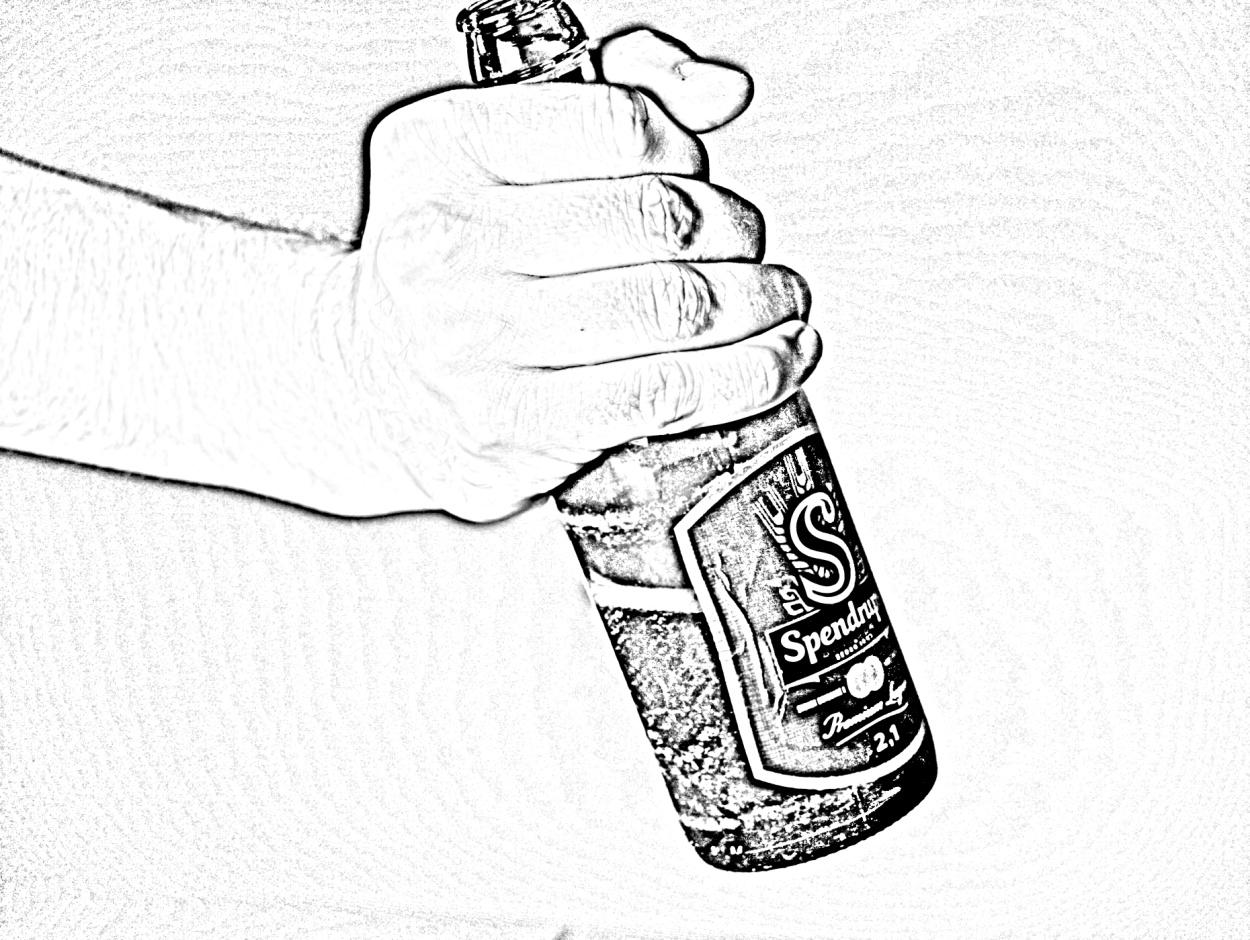
\includegraphics[width=1.0\textwidth]{res/olvisor.jpg}
   \section{Ölvisor}
\end{center}
\vfill
\newpage


\subsection{Hästhandlarn}
\textit{Mel: I ett hus vid skogens slut}\\
\textit{Vinnande ölvisa, Lundakarnevalen 1994}\\
\index[alfa]{Hästhandlarn}
\index[anfa]{Ur ett glas vid bordets slut...}
\begin{parse lines}[\noindent]{#1\\}

Ur ett glas vid bordets slut
liten starköl rinner ut
Lennart stirrar på sitt stop
bryter nog ihop
Nej, han vaknar ur sin nöd
cyklar hem till Veberöd
pantsätter sin systers föl
tusen spänn till öl
\end{parse lines}


\subsection{Öl!}
\textit{Mel: Var nöjd med allt som livet ger}\\
\index[alfa]{Öl"!}
\index[anfa]{Jag gillar alla sorters öl...}
\begin{parse lines}[\noindent]{#1\\}

Jag gillar alla sorters öl,
jag dricker dem med glädjebröl,
till frukost, lunch och middag varje dag!
Jag gillar öl för vet du vad?
Av bordsvatten blir ingen glad.
Nej, öl för fulla muggar vill jag ha.
\end{parse lines}

\newpage
\subsection{Strejk på Pripps}
\textit{Mel: I natt jag drömde}\\
\index[alfa]{Strejk på Pripps}
\index[anfa]{Inatt jag drömde något som...}
\begin{parse lines}[\noindent]{#1\\}

Inatt jag drömde något som,
jag aldrig drömt förut
Jag drömde det var strejk på Pripps
och alla ölen var slut.
Jag drömde om en jättesal
där ölen stod på rad
Jag drack sådär en femton
öl och reste mig och sa:
``Man kan ha roligt utan sprit,
men det är dumt att chansa.''
\end{parse lines}

\vspace{-0.2cm}
\subsection{Vi älskar öl}
\textit{Mel: Ser du stjärnan i det blå}\\
\index[alfa]{Vi älskar öl}
\index[anfa]{Täckt av silver sejdeln full...}
\begin{parse lines}[\noindent]{#1\\}

Täckt av silver sejdeln full
gnistrar mot oss med sitt guld
humle, malt, är livets salt, vi älskar öl.

Källarsval så bärs den in
för att glädja gommen din
släcka törsten, stärka rösten, till dess lov.

Knubbig blir du, men so what
gott och roligt har du fått
extra turen, rensat njuren, öl är gott.
\end{parse lines}

\vspace{-1cm}
\subsection{Öl-kanon}
\textit{Mel: Row, row, row your boat}\\
\index[alfa]{Öl-kanon}
\index[anfa]{Drick, drick, drick din öl...}
\begin{parse lines}[\noindent]{#1\\}

Drick, drick, drick din öl
låt den rinna ner.
Kan du sen kraxa
``en laxask med slasktratt''
så får du dricka fler.
\end{parse lines}


\subsection{Ont i Huvudet}
\textit{Mel: Ingeborg}\\
\index[alfa]{Ont i Huvudet}
\index[anfa]{Om du har ont i huvet...}
\begin{parse lines}[\noindent]{#1\\}

Om du har ont i huvet
när du vaknar någon da
så häll en öl i håret
och låt den stå och dra.

Och känns det inte bättre
så skyll inte på oss,
Att hälla öl i huvet
är inte smart förstås.
\end{parse lines}


\vfill
\subsection{Ode till ölet}
\textit{Mel: Trampa på gasen}\\
\index[alfa]{Ode till ölet}
\index[anfa]{Tu tu tu Tuborg...}
\begin{parse lines}[\noindent]{#1\\}

Tu tu tu Tuborg
och ca ca ca Carlsberg
det är den bästa
pi pi pi pilsnern som jag vet

Tu tu tu Carlsberg
och ca ca ca Tuborg
det är det bästa
pi pi pi ölet som jag vet

Tu tu tu Ölberg
och ca ca ca Pilsborg
det är den bästa
pi pi pi biran som jag vet

Tu ca pi Ölsner
och pi tu ca bira
det är den bästa
ca pi tu lering som jag gjort
\end{parse lines}




\vfill
\subsection{Om en söt dryck}
\textit{Mel: En tokig sång}\\
\index[alfa]{Om en söt dryck}
\index[anfa]{Jag dricker gärna öl och vin...}
\begin{parse lines}[\noindent]{#1\\}

Jag dricker gärna öl och vin
till sillen tar jag nubben
och kanske till och med en shot
när jag har gått till klubben.

Men drycken som jag helst vill ha
den har så friska lukter
den är dessutom ren och klar
och smakar utav frukter

Hå hum, man é ej dum
för att man dricker cider
Även om, det finnes dom
som utav smaken lider

Det skummar upp i glaset när
man har hällt upp en cider
det smakar både sött och gott
när den i halsen glider

Det kan vá både söt och torr
av tranbär eller fläder
av plommon och det finns nån sort
som smakar gamla kläder

Hå hum, man é ej dum...
\end{parse lines}

\vspace{-0.9cm}
\subsection{Ölets kretslopp}
\textit{Mel: Auld Lang Syne}\\
\textit{Vinnande bidrag bordsvisesittning 2018}\\
\index[alfa]{Ölets kretslopp}
\index[anfa]{Om någon gång du spillt din öl...}
\begin{parse lines}[\noindent]{#1\\}

Om någon gång du spillt din öl
Och gråtit över det
Om någon gång du spillt din öl
Då hoppas jag du vet

Att vattnet har ett kretslopp som
För ölen upp i sky
$\vert\vert$: Så nästa gång som regnet kom
Bli full på homeopati :$\vert\vert$
\end{parse lines}
\vfill
\noindent\textit{De sista två raderna kan sjungas X antal gånger där $2\leq$ X $\leq$ $ \sim33$.}

\newpage
\subsection{Udflykt til Danmark}
\textit{Mel: Mitt lilla fejs och jag}\\
\textit{K-sektionen Sångarstriden 1992}\\
\index[alfa]{Udflykt til Danmark}
\index[anfa]{Om du har det trist i Lund...}
\begin{parse lines}[\noindent]{#1\\}

Om du har det trist i Lund,
åk över Öresund.
Sätt dig på en färja,
sen så kan du härja.
Köp en öl, köp en till
eller Köpenhamn
köp så mycket öl du vill,
smuggla om du kan.

Man kan se på konst, jovisst,
på Louisiana
men visst är det ganska trist,
bara gå och glana.
Så vi kör till Helsingör,
köper lite smör.
Heja Danmark friskt humör,
sjunger vi i kör.

Många søde piger finns,
dejligt sensuella
men man bör se upp med kvinns,
tänk på salmonella.
Lajbans hela natten lång,
festa som en vilde.
Rockmusik och hålligång,
värre än Roskilde.

Nästa morgon, nästan död,
står man där i tullen.
Näsan lyser vit och röd,
halsen den är svullen.
Jag ska smuggla kött och öl,
men vad smugglar du?
Och du svarar med ett bröl:
``Den lille havefrue!''
\end{parse lines}


\subsection{Prostatabesvär}
\textit{Mel: I Apladalen i Värnamo}\\
\index[alfa]{Prostatabesvär}
\index[anfa]{Jag kissar inte nån fin parabel...}
\begin{parse lines}[\noindent]{#1\\}

Jag kissar inte nån fin parabel.
Jag har fått nått hinder uti min snabel.
Ja, dricka öl ställer till besvär,
med en prostata som denna här.
\end{parse lines}


\newpage

\subsection{Ölen är slut}
\textit{Mel: Havet är djupt}\\
\index[alfa]{Ölen är slut}
\index[anfa]{Det börjar bli sent på festen...}
\begin{parse lines}[\noindent]{#1\\}

Det börjar bli sent på festen
och alla har jävligt kul.
Du slog din rival på beerpong
och din dans börjar bli ful.

Men du kan ej begripa
rösten som kallar ut.
``Det där var vår sista IPA
och nu så är ölen slut!''
Åh nej!

Ölen är slut!
Ölen är slut!
Ända till Lomma,
är burkarna tomma.
Ölen är slut!
I kylskåpet finns ju ingenting,
förutom tacos och powerking.
Så om du vill halsa,
nöj dig med salsa.
Ölen är slut!

Hos grannen är alla glada,
dit floder av IPA når,
men här på efterfesten
rinner endast en tår.
Du mister ditt lugn i krisen
och slutar att vara snäll.
Sen cakear du på polisen
och hamnar i fyllecell.
Åh nej!

Ölen är slut!
Ölen är slut!
Så drick mer vatten,
sov gott om natten,
sen pustar vi ut.
I kylskåpet finns ju ingenting,
förutom tacos och powerking.
Så om du vill halsa,
nöj dig med salsa.
Ölen är slut!
\end{parse lines}

\newpage
